\documentclass[11pt,oneside]{article}	%use"amsart"insteadof"article"forAMSLaTeXformat
\usepackage{geometry}		%Seegeometry.pdftolearnthelayoutoptions.Therearelots.
\geometry{letterpaper}		%...ora4paperora5paperor...
%\geometry{landscape}		%Activateforforrotatedpagegeometry
%\usepackage[parfill]{parskip}		%Activatetobeginparagraphswithanemptylineratherthananindent
\usepackage{graphicx}				%Usepdf,png,jpg,orepsßwithpdflatex;useepsinDVImode
								%TeXwillautomaticallyconverteps-->pdfinpdflatex		
\usepackage{amssymb}
\usepackage[colorlinks]{hyperref}

%----macros begin---------------------------------------------------------------
\usepackage{color}
\usepackage{amsthm}

\def\conv{\mbox{\textrm{conv}\,}}
\def\aff{\mbox{\textrm{aff}\,}}
\def\E{\mathbb{E}}
\def\R{\mathbb{R}}
\def\Z{\mathbb{Z}}
\def\tex{\TeX}
\def\latex{\LaTeX}
\def\v#1{{\bf #1}}
\def\p#1{{\bf #1}}
\def\T#1{{\bf #1}}

\def\vet#1{{\left(\begin{array}{cccccccccccccccccccc}#1\end{array}\right)}}
\def\mat#1{{\left(\begin{array}{cccccccccccccccccccc}#1\end{array}\right)}}

\def\lin{\mbox{\rm lin}\,}
\def\aff{\mbox{\rm aff}\,}
\def\pos{\mbox{\rm pos}\,}
\def\cone{\mbox{\rm cone}\,}
\def\conv{\mbox{\rm conv}\,}
\newcommand{\homog}[0]{\mbox{\rm homog}\,}
\newcommand{\relint}[0]{\mbox{\rm relint}\,}

%----macros end-----------------------------------------------------------------

\title{Boundary operators on LAR
\footnote{This document is part of the \emph{Linear Algebraic Representation with CoChains} (LAR-CC) framework~\cite{cclar-proj:2013:00}. \today}
}
\author{Alberto Paoluzzi}
%\date{}							%Activatetodisplayagivendateornodate

\begin{document}
\maketitle
\nonstopmode

\begin{abstract}
The various versions of boundary operators on Linear Algebraic Representation of cellular complexes are  developed in this module, in order to maintain under focus their proper development, including the possible special cases.
\end{abstract}

\tableofcontents
\newpage

\section{Introduction}

In the current \texttt{LarLib} implementation, we have to distinguish between between dimension-independent, dimension-dependent, signed and non-signed operators.
Therefore a refactoring of the \texttt{LarLib} code related to boundary/coboundary operators started here, with the aim to provide a precise mathematical definition witin the LAR framework, and to simplify and generalise the related algorithms.


\section{Implementation}

We start this section by making a distinction between 


\subsection{Non-signed operators}


\subsubsection{Dimension-independent}


\paragraph{Convex-cells}

%-------------------------------------------------------------------------------
@D convex-cells boundary operator
@{""" convex-cells boundary operator """
from larcc import *
def boundary(cells,facets):
    lenV = max(CAT(cells))+1
    csrCV = csrCreate(cells,lenV)
    csrFV = csrCreate(facets,lenV)
    csrFC = matrixProduct(csrFV, csrTranspose(csrCV))
    facetLengths = [csrCell.getnnz() for csrCell in csrCV]
    return csrBoundaryFilter(csrFC,facetLengths)
@}
%-------------------------------------------------------------------------------


\paragraph{Path-connected cells}

%-------------------------------------------------------------------------------
@D path-connected-cells boundary operator
@{""" path-connected-cells boundary operator """
import larcc
from larcc import *
def boundary1(CV,FV,EV):
    lenV = max(CAT(CV))+1
    csrCV = csrCreate(CV,lenV)
    csrFV = csrCreate(FV,lenV)
    csrFC = matrixProduct(csrFV, csrTranspose(csrCV))
    facetLengths = [csrCell.getnnz() for csrCell in csrCV]
    VV = AA(LIST)(range(lenV))
    csrBBMat = boundary(FV,EV)*boundary(CV,FV)
    FE = larcc.crossRelation(lenV,FV,EV,True)
    return csrBoundaryFilter1(csrBBMat,CV,FV,EV,lenV,FE,csrFC,facetLengths)
@}
%-------------------------------------------------------------------------------

\subsection{Signed operators}


\section{Exporting}

%-------------------------------------------------------------------------------
@O larlib/larlib/boundary.py
@{""" boundary operators """
from larlib import *
@< convex-cells boundary operator @>
@< path-connected-cells boundary operator @>
@}
%-------------------------------------------------------------------------------


\section{Testing}

\section{Non-signed operators}


%-------------------------------------------------------------------------------
@O test/py/boundary/test01.py
@{""" testing boundary operators """
from larlib import *

filename = "test/svg/inters/boundarytest0.svg"
lines = svg2lines(filename)
VIEW(STRUCT(AA(POLYLINE)(lines)))
    
V,FV,EV,polygons = larFromLines(lines)
VV = AA(LIST)(range(len(V)))
submodel = STRUCT(MKPOLS((V,EV)))
VIEW(larModelNumbering(1,1,1)(V,[VV,EV,FV],submodel,0.2))
VIEW(EXPLODE(1.2,1.2,1.2)(MKPOLS((V,[EV[e] for e in boundaryCells(FV,EV)],))))
VIEW(EXPLODE(1.2,1.2,1.2)(MKTRIANGLES((V,FV,EV))))

boundaryOp = boundary(FV,EV)

for k in range(1,len(FV)+1):
    faceChain = k*[1]
    BF = chain2BoundaryChain(boundaryOp)(faceChain)
    VIEW(STRUCT(MKPOLS((V,[EV[e] for e in BF]))))
@}
%-------------------------------------------------------------------------------

%-------------------------------------------------------------------------------
@O test/py/boundary/test02.py
@{""" testing boundary operators """
from larlib import *

filename = "test/svg/inters/boundarytest1.svg"
lines = svg2lines(filename)
VIEW(STRUCT(AA(POLYLINE)(lines)))
    
V,FV,EV,polygons = larFromLines(lines)
VV = AA(LIST)(range(len(V)))
submodel = STRUCT(MKPOLS((V,EV)))
VIEW(larModelNumbering(1,1,1)(V,[VV,EV,FV],submodel,0.2))
VIEW(EXPLODE(1.2,1.2,1.2)(MKPOLS((V,[EV[e] for e in boundaryCells(FV,EV)],))))
VIEW(EXPLODE(1.2,1.2,1.2)(MKTRIANGLES((V,FV,EV))))

boundaryOp = boundary(FV,EV)

for k in range(1,len(FV)+1):
    faceChain = k*[1]
    BF = chain2BoundaryChain(boundaryOp)(faceChain)
    VIEW(STRUCT(MKPOLS((V,[EV[e] for e in BF]))))
@}
%-------------------------------------------------------------------------------

\begin{figure}[htbp] %  figure placement: here, top, bottom, or page
   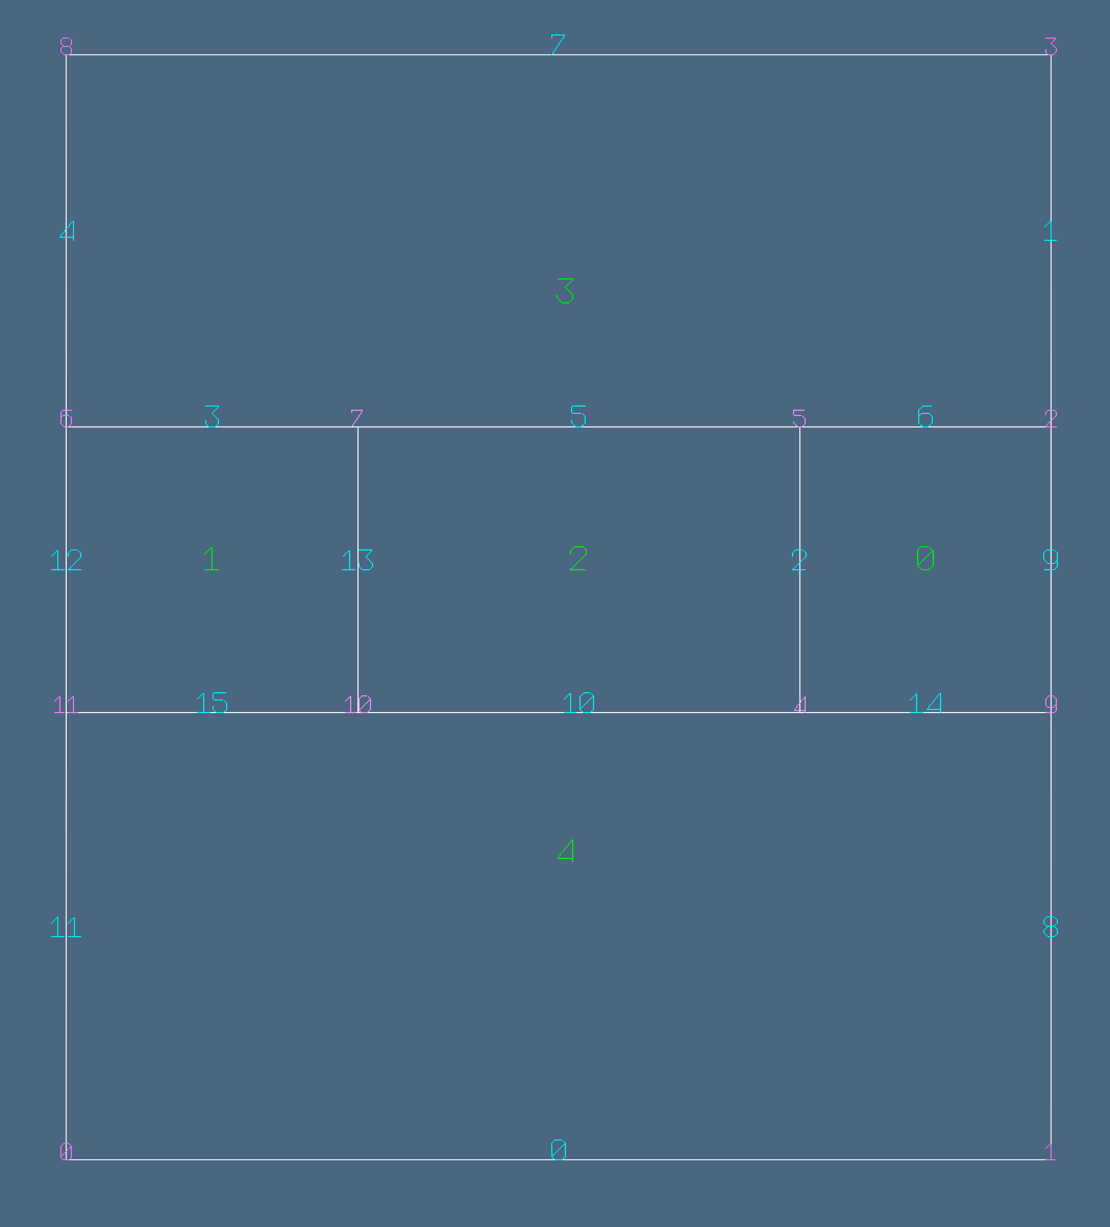
\includegraphics[height=0.245\linewidth,width=0.245\linewidth]{images/boundary-test01-2} 
   
\includegraphics[height=0.245\linewidth,width=0.245\linewidth]{images/boundary-test01-3} 
   
\includegraphics[height=0.245\linewidth,width=0.245\linewidth]{images/boundary-test01-4} 
   
\includegraphics[height=0.245\linewidth,width=0.245\linewidth]{images/boundary-test01-5} 

   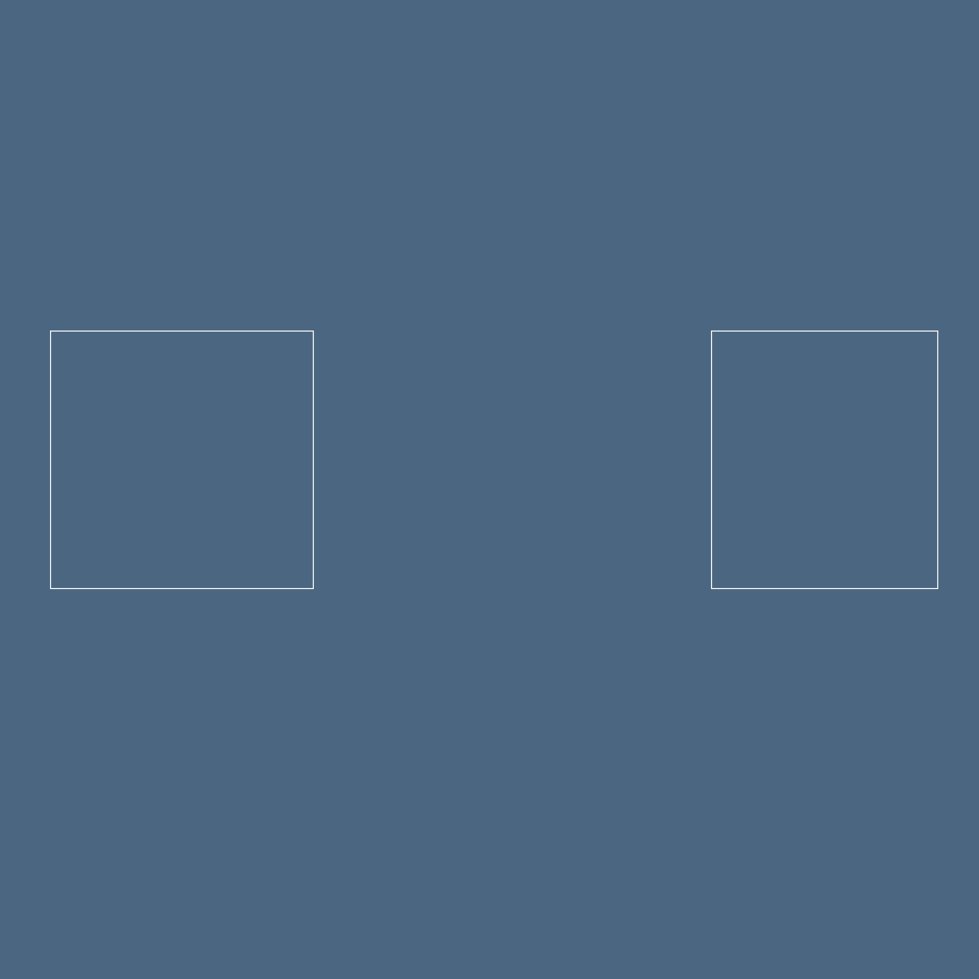
\includegraphics[height=0.245\linewidth,width=0.245\linewidth]{images/boundary-test01-6} 
   
\includegraphics[height=0.245\linewidth,width=0.245\linewidth]{images/boundary-test01-7} 
   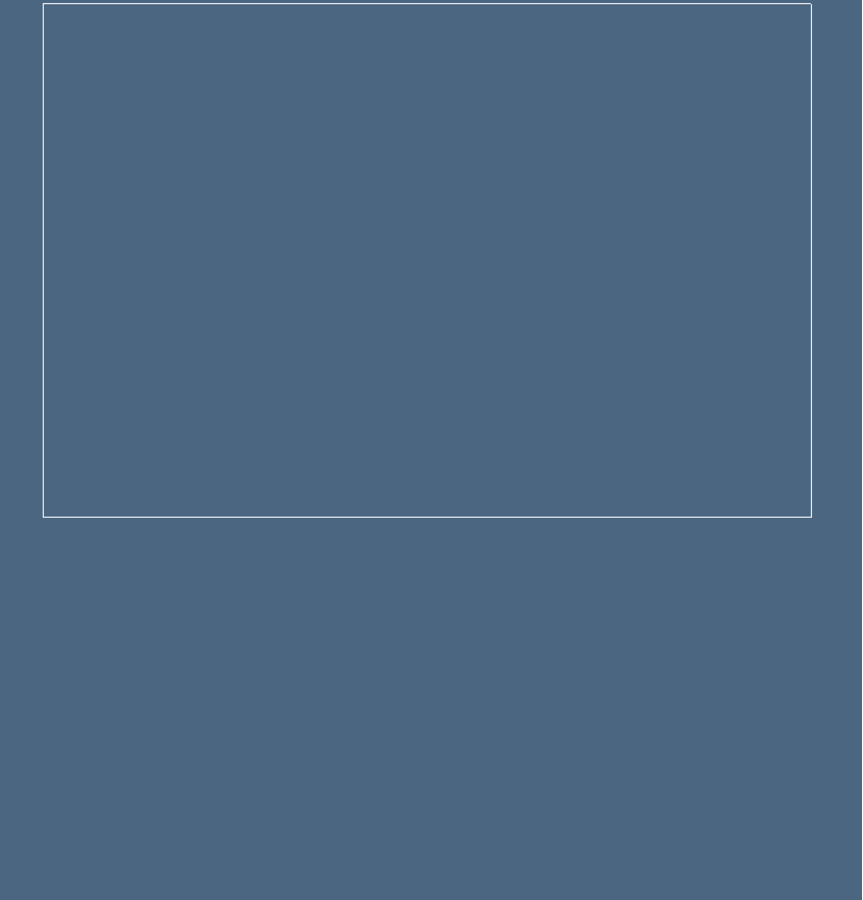
\includegraphics[height=0.245\linewidth,width=0.245\linewidth]{images/boundary-test01-8} 
   
\includegraphics[height=0.245\linewidth,width=0.245\linewidth]{images/boundary-test01-9} 
   \caption{Convex-cell 2-complex. (a) Indexing of 0-,1-,and 2-cells; (b) exploded 2-boundary cells; (c) exploded 2-cells; (d) boundary of a singleton 2-chain; (e--f) boundaries of some 2-chains.}
   \label{fig:example}
\end{figure}


\begin{figure}[htbp] %  figure placement: here, top, bottom, or page
   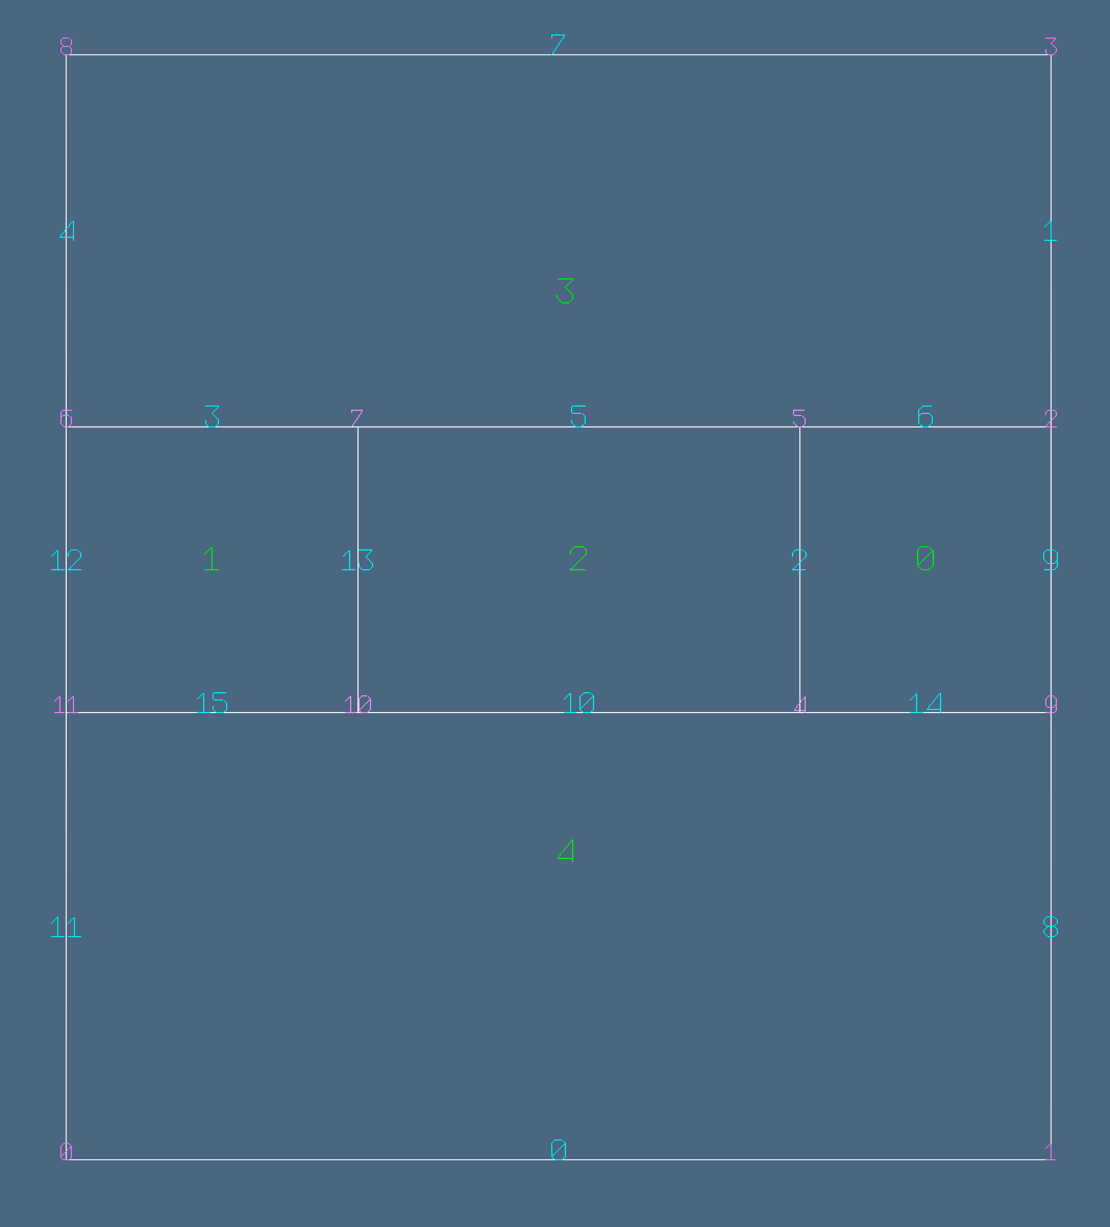
\includegraphics[height=0.245\linewidth,width=0.245\linewidth]{images/boundary-test01-2} 
   
\includegraphics[height=0.245\linewidth,width=0.245\linewidth]{images/boundary-test01-3} 
   
\includegraphics[height=0.245\linewidth,width=0.245\linewidth]{images/boundary-test01-4} 
   
\includegraphics[height=0.245\linewidth,width=0.245\linewidth]{images/boundary-test01-5} 

   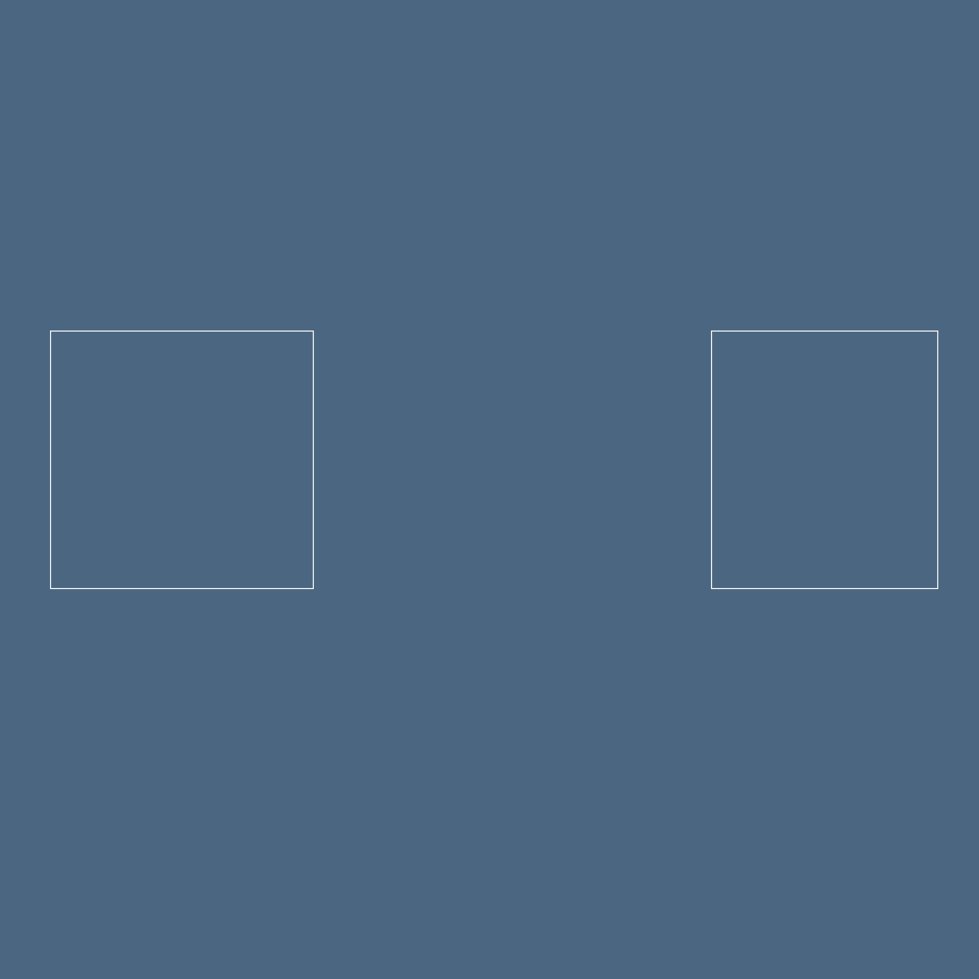
\includegraphics[height=0.245\linewidth,width=0.245\linewidth]{images/boundary-test01-6} 
   
\includegraphics[height=0.245\linewidth,width=0.245\linewidth]{images/boundary-test01-7} 
   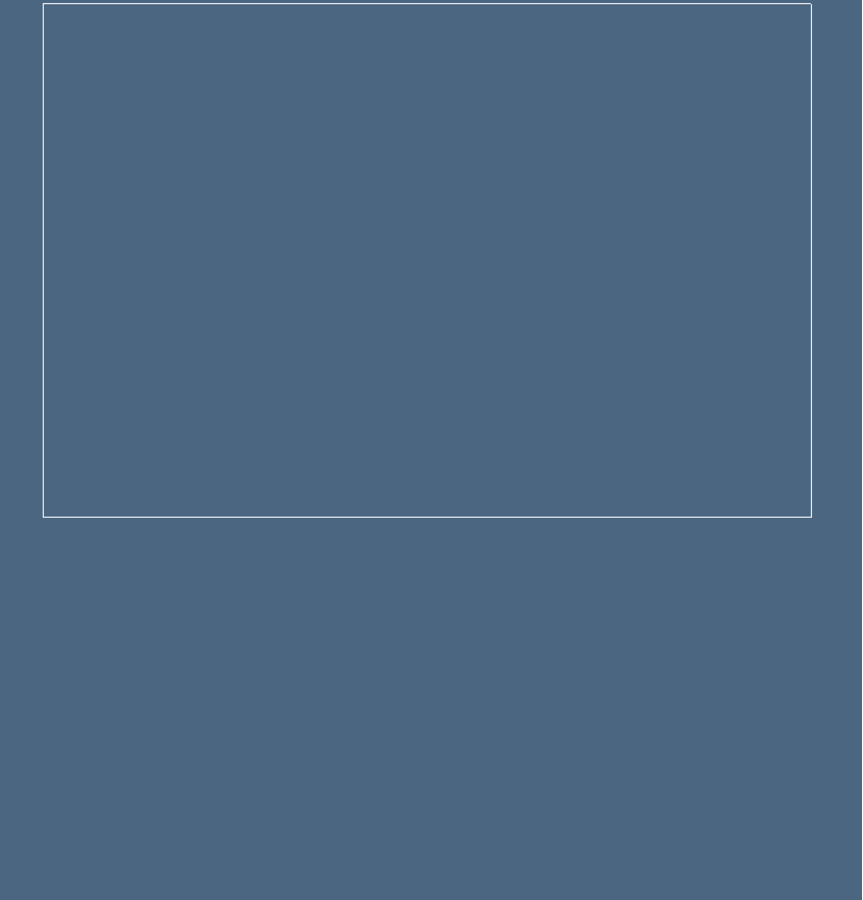
\includegraphics[height=0.245\linewidth,width=0.245\linewidth]{images/boundary-test01-8} 
   
\includegraphics[height=0.245\linewidth,width=0.245\linewidth]{images/boundary-test01-9} 
   \caption{A non-working example with \texttt{function}. (a) Indexing of 0-,1-,and 2-cells; (b) exploded 2-boundary cells; (c) exploded 2-cells; (d) boundary of a singleton 2-chain; (e--f) boundaries of some 2-chains.}
   \label{fig:example}
\end{figure}

\bibliographystyle{amsalpha}
\bibliography{boundary}

\end{document}
